\documentclass{article}

\usepackage{xcolor}
\usepackage{graphics}
\usepackage{graphicx}
\usepackage{hyperref}
%% added this package for math symbols and boxes
\usepackage{tikz}

\usepackage[utf8]{inputenc}
\usepackage{calligra}
\usepackage{amsmath}   
\usepackage{amssymb}
\usepackage{wasysym}
\usepackage{mathrsfs}
\usepackage{listings}
%defining tab
\newcommand\tab[1][1cm]{\hspace*{#1}}


\usepackage{titlesec}%%to avoid 'Chapter N'
\titleformat{\chapter}[display]
{\normalfont\bfseries}{}{0pt}{\Large}
\usepackage{fancyhdr}


\usepackage{listings}
\usepackage{color}
\usepackage{textcomp}

 \definecolor{vgreen}{RGB}{104,180,104}
\definecolor{vblue}{RGB}{49,49,255}
\definecolor{vorange}{RGB}{255,143,102}
\lstdefinestyle{verilog-style}
{
	language=Verilog,
	basicstyle=\small,
	keywordstyle=\color{vblue},
	identifierstyle=\color{black},
	commentstyle=\color{vgreen},
	numbers=left,
	upquote=true,
	aboveskip={1.5\baselineskip},
	columns=fixed,
	showstringspaces=false,
	extendedchars=true,
	breaklines=true,
	prebreak = \raisebox{0ex}[0ex][0ex]{\ensuremath{\hookleftarrow}},
	numberstyle={\tiny \color{black}},
	numbersep=10pt,
	tabsize=8
}


\lstdefinestyle{CStyle}{
	%backgroundcolor=\color{backgroundColour},   
	commentstyle=\color{mGreen},
	keywordstyle=\color{magenta},
	%numberstyle=\tiny\color{mGray},
	stringstyle=\color{mPurple},
	basicstyle=\footnotesize,
	breakatwhitespace=false,         
	breaklines=true,                 
	captionpos=b,                    
	keepspaces=true,                 
	%numbers=left,                    
	%numbersep=5pt,                  
	showspaces=false,                
	showstringspaces=false,
	showtabs=false,                  
	tabsize=2,
	language=C
}



\pagestyle{fancy}
\fancyhead[L]{\rightmark}
\rhead{EE712\_2019\_27 }
\lhead{Wireless DSO}
\cfoot{\thepage}
\renewcommand{\headrulewidth}{0.4pt}
\renewcommand{\footrulewidth}{0.4pt}

\begin{document}
	\author{by \endline Ananda Kundu	(18307R025)	 anandakundu13@gmail.com 
		\endline Aswin P Ajayan	(183079032) 	aswinp2008@gmail.com
		\endline Sunny Mehta	(183079023) 	sunnymehta78669@gmail.com}
	\title{Wireless DSO}
	\maketitle
	
	\section{Abstract}
	The project aims at creating wireless DSO modules for measuring differential voltage
	signals with high common mode signals, observing signal variations and waveforms
	and monitoring them from a remote location.
	We implemented a circuit to get the differential output without inputs getting
	overloaded by common mode signal. For this purpose, common mode signal is
	attenuated to avoid the saturation of output, both the inputs are separately
	attenuated and get the differential signal. But recognizing in the process of
	attenuating the common mode signal, differential signal is also getting attenuated,
	and so need to be amplified the differential signal.
	\begin{figure}
		\centering
		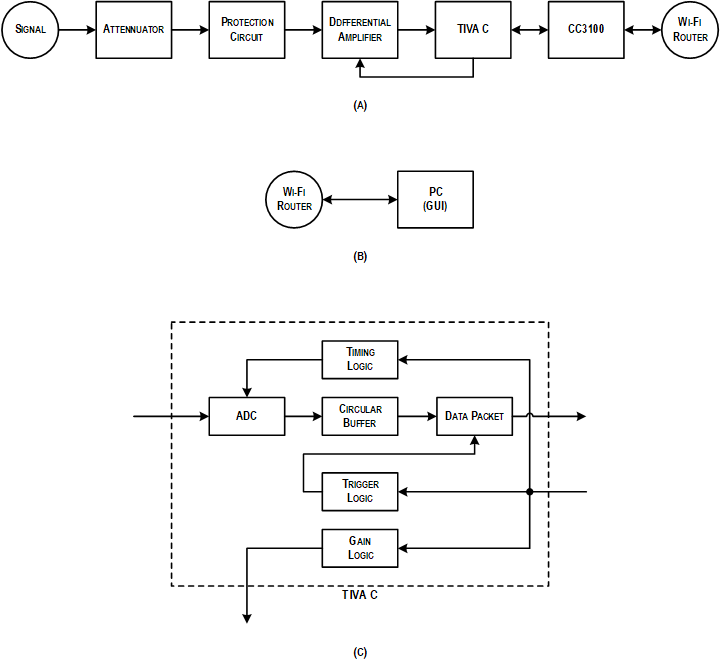
\includegraphics[width=0.7\linewidth]{BlockDiagram}
		\caption{Block Diagram: a,b) hardware blocks c)logical blocks}
		\label{fig:blockdiagram}
	\end{figure}
	
	
	\section{Introduction}
	The measurements usually made using normal oscilloscope probes are single
	ended, that is the low line of the probe is connected to ground and the high line is
	connected to test node. If it is needed to make differential measurement, then both
	the channels of scope were used and make single ended measurements of two test
	points with respect to ground and by subtraction operation the difference signal is
	measured. Though with this technique the purpose is solved, it needs two CRO
	channels to make a single differential measurement. With a differential probe, the
	differential measurement can be made with the help of a single channel. Another
	advantage of using differential probe is it can measure differential output with very
	high common mode without saturating.
	The differential signal is then converted to fit the ADC range (0-3.3 V) using the
	circuit described later. This signal is then given to the ADC port of TIVA C launchpad
	which has an inbuilt ADC with 10-bit resolution. The data from ADC is then sent to
	the PC via Wi-Fi using CC3100. The data received by the PC is used to plot the
	signal in GUI. In GUI we had included three sliders to control voltage scaling, time
	scaling and level triggering.
	
	\section{Circuit Description}
	\subsection{Reference Generator}
	The circuit comprises of op-amp and POT as shown in schematic. As we are
	using a single ended power supply (0-5 V), this is required to generate a ground
	reference for the amplification stage.
	We used POT instead of resistors so that we can calibrate the output for zero.
	\subsection{Attenuator}
	\begin{figure}
		\centering
		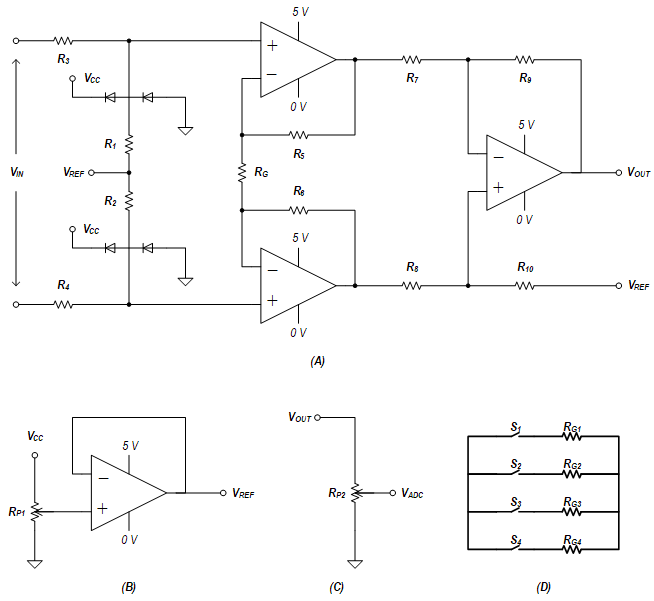
\includegraphics[width=0.7\linewidth]{Schmatic1}
		\caption{a) Diff Amplifier with input attnennuator and protection circuit b) refernce voltage generator c) output attennuator d) Rg for variable gain}
		\label{fig:schmatic1}
	\end{figure}
	
	The attenuator is used in the input side so that signals with larger peak to
	peak values can be plotted. It will increase the dynamic range of our system.
	\subsection{Protection circuit}
	A diode protection circuit is implemented as shown in the schematic; its purpose
	is to prevent the input of the amplifier stage going beyond the supply voltages. This
	protects the op-amp circuitry from any over voltages.
	\subsection{Differential amplifier with variable gain}
	We have used instrumentation amplifier over general differential amplifier, as
	it has better CMRR. Further, we have used INA118 as it has inbuilt overvoltage
	protection and better output swing.
	We have used analog switch (4066), to vary the resistor R g , which in turn
	varies the gain
	\subsection{Output attenuator}
	At output stage we have connected a POT as an attenuator to match the
	output range (0-5 V) of the amplifier stage with the input range (0-3.3 V) of the ADC.
	
	\begin{figure}[!]
		\centering
		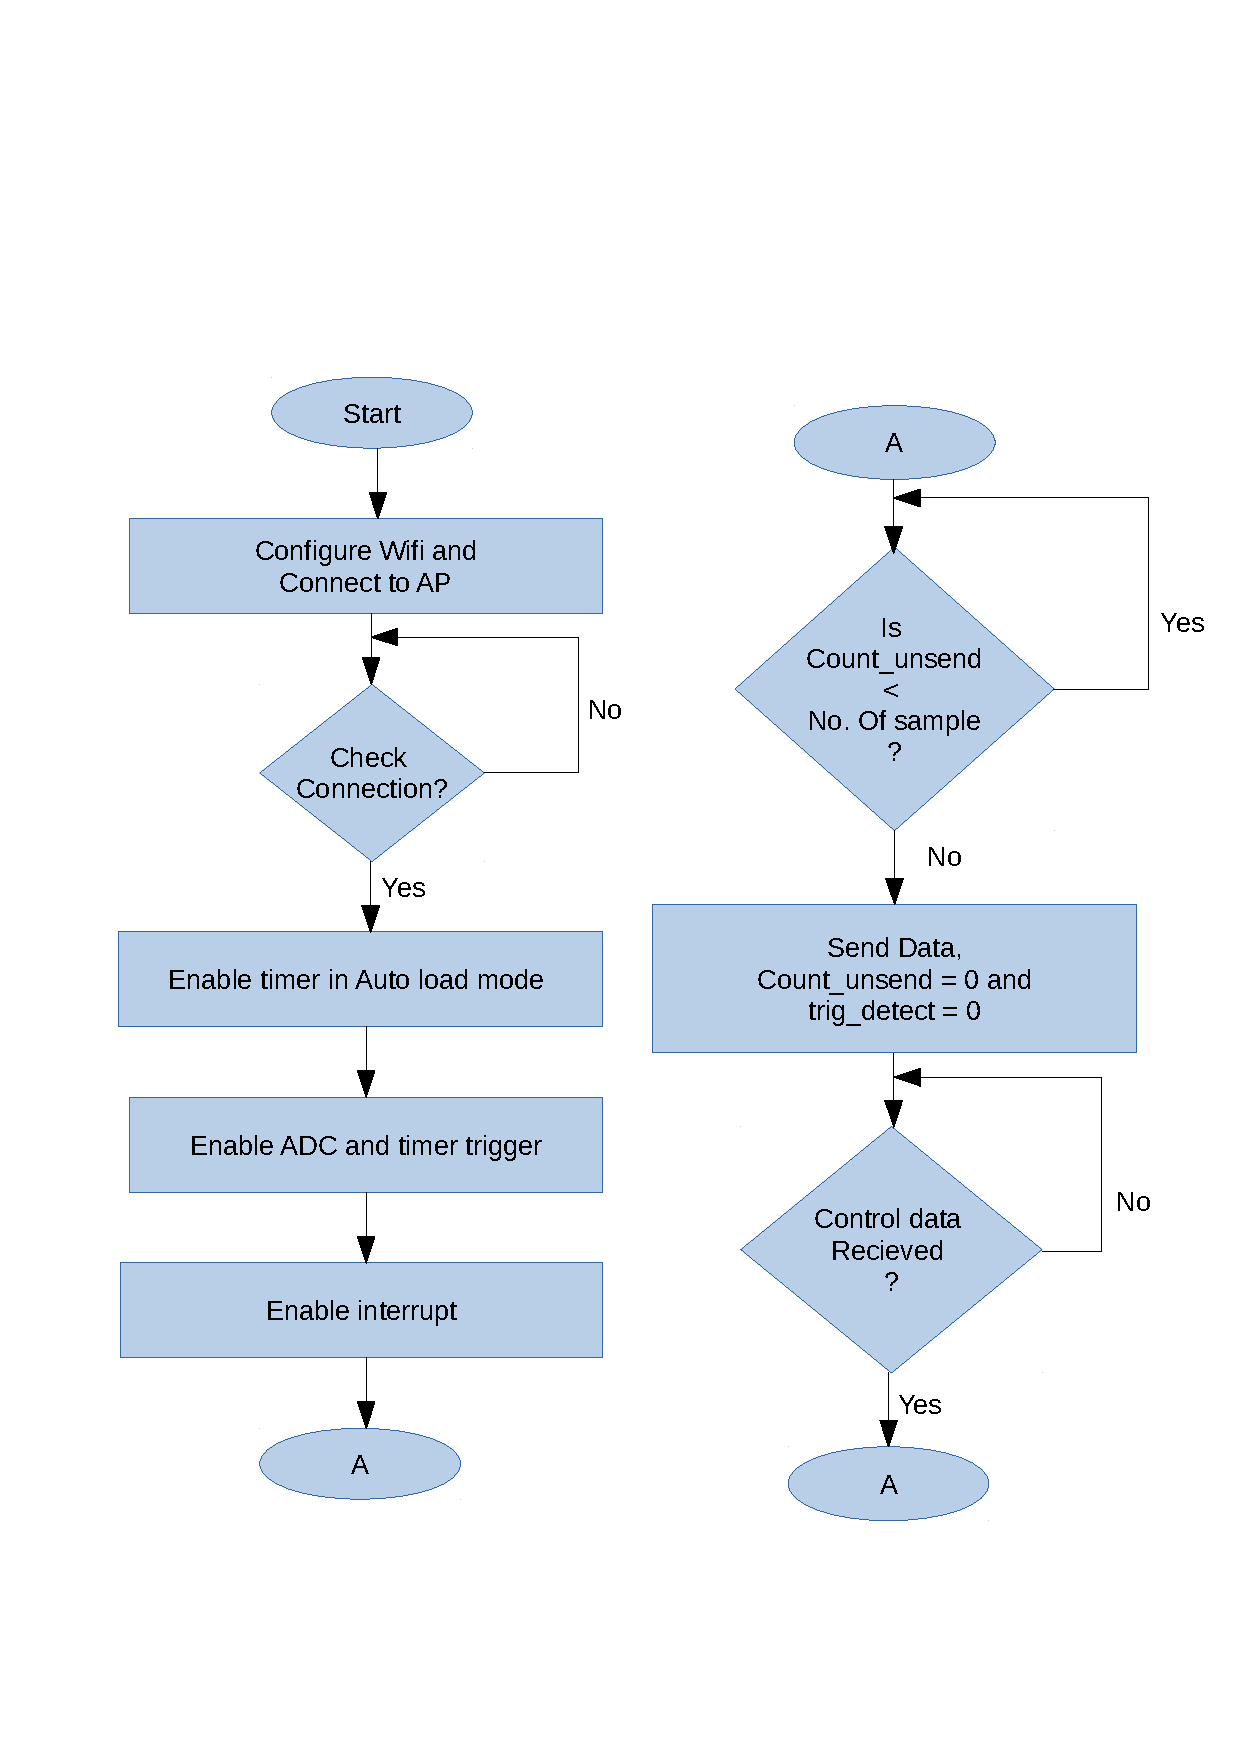
\includegraphics[width=0.7\linewidth]{flowchart_main}
		\caption{}
		\label{fig:flowchartmain}
	\end{figure}


	\begin{figure}[!]
		\centering
		\includegraphics[width=0.7\linewidth]{"report embedded3"}
		\caption{Flowchart: interrupt handler}
		\label{fig:report-embedded3}
	\end{figure}
	



	\section{Controller and Firmware }
	We chose Tiva C Launchpad board for our project. It uses \textbf{TM4C1236GHPM} MCU . It doesn't have embedded wifi capabilities , so we were using \textbf{CC3100} add on board for the same .  has 2 inbuilt ADC's. TM4C123GH6PM has in-built ADC module with sampling frequency approaching 1 Mega samples per second and with a resolution of 12 bits . It supports various triggering modes.
	\subsection{Sampling and Timing}
	In any Oscilloscope, the task of  setting up correct sampling interval is of utmost importance. To ensure that stringent timing requirements are met  ADC was configured in \textit{timer triggered} mode .  Inbuilt
	ADC module in TM4C123GH6PM was used.Given below are the cofigurations used by us for setting up the sampler\\\\
	ADC Channel			: ADC\_CTL\_CH4\\
	Triggering mode : Timer Trigger	\\	
	Sampling Freq 	: 512 kHz (varied later by downsampling)\\\\
	Timer A is configured to generate periodic interrupts at a rate of 512 kHz which inturn triggers the ADC 
	module.\\ source files : \textit{Timing  and ADC configuration  main.c}\\ 
	\textit{Interrupt handler needs are enabled in tm4c123gh6pm\_startup\_ccs.c}
	\subsection{Circular buffer and Triggering}
	The sampled data is then stored in a circular buffer of size 512 * 16(see to timing control section ). The value is set by the macro
	\begin{lstlisting}[style=CStyle]
	#define NO_OF_SAMPLES 16384
	\end{lstlisting}
	A seperate buffer of the same size is kept for taking the first order difference as 
	\begin{lstlisting}[style=CStyle]
	diff_buf[i] = inb_buf[i] - in_buf[i-1]
	\end{lstlisting}
	At the time of sampling itself, the sampled value is checked for a \textbf{trigger level} (set from ui) and a caliberated difference value in diff buf(to distinguish edges). once the trigger is detected a \textbf{counter is incremented for every sample acquired} . The process is continued till the counter exceeds the NO\_OF\_SAMPLES. After that the interrupt is disabled and \textbf{DATA PACKET} is pushed to the server (laptop) and waits for the reply back from laptop. Once the Controller receives the data from computer it reconfigures the sampler and re-enables the interrupt. And the cycle continues. \\
	\textit{When the trigger condition is not detected till a specified pre-defined threshold , it sends the data captured to the Laptop without any synchronisation. Thus resulting in a running wave form.(see trigger control)}
	
	\subsection{Wifi Connection and UDP Client }
	Tiva provides seperate SDK for their wifi modules. In our case it was the \textbf{CC3100 SDK} . (basically the simple link driver library). We builded upon the \textit{getting\_started\_with\_wlan\_ap}. The MCU can be programmed to be in Station Mode or access point mode( \textit{sl\_common.h}). When acting as station it gets connected to the router using the SSID and password specified in sl\_common.h\\
	
	To communicate data over Wi-fi we are using UDP protocol. The MCU acts as a UDP client and PC acts as UDP server . \textit{IP\_ADDRESS} of the laptop  and the \textit{PORT} needs to be specified in main.c
	
	\section{DSO-User-Interface and UDP Server }
	\begin{center}
	\begin{tabular}{ll}

		\hline 
		C Libararies Used &  \\ 
		\hline 
		User Interface & gtk 3  \\ 
	 
		Plotting Wave form & cairo \\ 
	
		Multi Threading & pthreads \\ 
	
		UDP & linux system libraries \\ 
		\hline 
	\end{tabular} 
	\end{center}
	Since the UDP server side uses linux system libraries, the ui might work in linux systems only.\\
	The program for UI is purely event driven. Various events and controls in ui are described as in the following sections
	\subsection{Connect Button:} 
	The botton spawns two threads , UDP socket thread and Async Plotter.
	
	Multithreading ensures the responsivity of UI
	
	
	\subsection{Redraw Button:} 
	The button is to replot the graph ion case when the user interface is stuck.
	\begin{figure*}
		\centering
		\includegraphics[width=1.2\linewidth]{"Screenshot from 2019-05-06 16-06-52"}
		\caption[ee712_Scope]{Oscilloscope Ui depicting the features}
		\label{fig:screenshot-from-2019-05-06-16-06-52}
	\end{figure*}
	\subsection{Export Button:}
	The button is used to invoke the function to collect the samples recived and save them in a .csv file.
	The data can be used to check the plot observed or as a saved analysis.
	
	\subsection{Threads}
	\begin{lstlisting}[style=CStyle]
	void* socketThread(void *arg)
	\end{lstlisting}
	This thread implements a UDP socket server and waits for an incoming packet from MCU . Recieved data is copied to shared buffer. Then control data from UI is send back to the Micro controller . It triggers the async Plotter thread to start plotting the data. 
	\begin{lstlisting}[style=CStyle] 
	void* async_plotter_thread(void *arg);
	\end{lstlisting}
	Copies the data from shared buffer to a dedicated buffer and request the gtk drawing area for a redraw by invalidating the draw area
	\begin{lstlisting}[style=CStyle]
	gtk_widget_queue_draw(ui_pointer->w_drawing_area);
	\end{lstlisting}
	Redrawing of the ui is done by the function
	\begin{lstlisting}[style=CStyle]
	static void do_drawing(cairo_t *cr,double WIDTH,double HEIGHT)
	\end{lstlisting}
	
	\subsection{Voltage scale slider :}
	
	The slider can be used to change the voltage per division . By default it is set to the minimum value. The change in scale will send the gain value to the controller and the respective resistor value will be selected.The selection of 
	resistor is taken care by analog switch .
	
	\subsection{Time scale slider :}
	
	The slider can be used to change the time per division on the display.By default the sampling frequency is 512 Khz which is the maximum(for simplicity ). The change in scale will send the requried sampling frequency by the user and controller will take care of it based on the input recieved. Down sampling is done in the micro controller itself to reduce data transmission.
	
	\subsection{Trigger level slider :}
	On the interface , thje trigger slider can be used to trigger the waveform at a particular value.By defalut the trigger level is 0 V.To implement the trigger we are using 128 different levels to accomodate different 1024 voltage levels.The respective trigger value will be send to the controller before receiving the data to be plotted.
	\section{Source code}
	Source code for this project is spread across two public repositories in github\\
	User interface \href{https://github.com/aswinpajayan/ScopeUI.git}{ee712-Scope}\\
	Firmware for MCU \href{https://github.com/aswinpajayan/wifi-DSO-module.git}{firmware}
	
	\section{Conclusion}
	This wireless DSO module can be used for  measurements
	over Wi-Fi so that it can be observed anywhere in the range of Wi-Fi module. Further since we use UDP. The data can be sent to any node in an intranet. This will be helpful in carrying out filed measurements from a lab. 
	However, the features of DSO included in this project is very limited. Also, for
	increasing the range of frequencies that the DSO module can measure, an ADC with
	high sampling rate is recommended.
	Wi-Fi technology is used in this application. Hence it works about 10-100m at very
	high-speed data transmission of 10-105 MBps. Wi-Fi doesn’t consume high power
	compared to normal DSO. Now a days, tablet computers are used very much among
	people. When this GUI interface is once installed in the tablet computers, we can use
	whenever we are in need of Oscilloscope and its remote control is possible. Wi-Fi
	transmitter is also portable. And this interface also makes so easier to observe
	response of the circuit as graphical waveform.
	\section{References}
	\begin{itemize}
		\item \url{http://users.ece.utexas.edu/~valvano/arm/wirelessconnectivity.html}\\
		for making tiva board wifi connection
		\item \href{http://www.ti.com/lit/ug/spmu298d/spmu298d.pdf}{TIVA C peripheral library users manual}
		\item \url{https://www.geeksforgeeks.org/udp-server-client-implementation-c/}
		\item \url{https://www.gtk.org/documentation.php}
		\item \url{https://developer.gnome.org/gtk3/stable/gtk-getting-started.html}
		\item \url{https://www.cairographics.org/samples/}
		\item linux man pages
		
		
	\end{itemize}

	
	
	
	
	
	
	
	
	
    .................................................................
    ..................................................................
  


	
	
\end{document}